\documentclass[12pt, varwidth, border={20mm 5mm 5mm 20mm}]{standalone}
\usepackage{tikz}
\usepackage{amsmath}
\usepackage[a4paper, portrait, margin=1cm]{geometry}
\begin{document}
\section*{First Class Levers}
    \begin{minipage}{0.5\textwidth}
    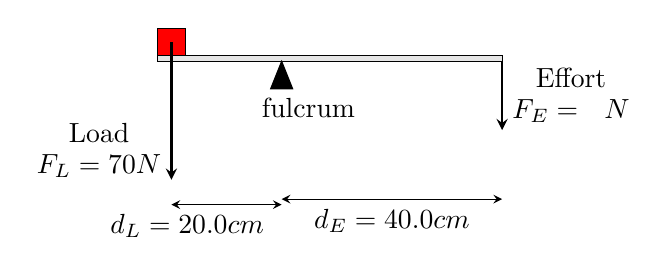
\begin{tikzpicture}[scale=0.7,>=stealth]
        % First class lever
        % rod
        \draw[fill=gray!20] (-0.25,0) rectangle (6,0.1);
        %fulcrum
        \draw[fill=black] (1.8,-0.5) -- (2.2,-0.5) node[below,xshift=2mm] {fulcrum} -- (2.0,0) -- cycle;
        %load
        \draw[fill=red] (-0.25,0.1) rectangle (0.25,0.6);
        \draw[->,thick] (0.0,0.35) -- (0.0,-2.15) node[midway,left,yshift=-0.5cm,align=center] {Load \\\\[-3ex] $F_L = 70N$};
        %effort
        \draw[->,thick] (6,0.0) -- (6,-1.25) node[midway,right,align=center] {Effort \\\\[-3ex] $F_E = ~~N$};

        % Distance markers
        \draw[<->] (2.0,-2.5) -- (6,-2.5) node[midway,below,align=center] {$d_E = 40.0cm$};
        \draw[<->] (0,-2.6) -- (2.0,-2.6) node[midway,below,xshift=-0.5cm,align=left] {$d_L = 20.0cm$};
    \end{tikzpicture}
\end{minipage}%
\hfill
\begin{minipage}{0.5\textwidth}
    \begin{flalign*}
        && F_E \times d_E &= F_L \times d_L && \\
        && F_E &= \frac{F_L \times d_L}{d_E} && \\
        && F_E &= \frac{~~ \times ~~}{~~} && \\
        && F_E &= ~~N &&
    \end{flalign*}
\end{minipage}
\end{document}
